\normchapter{Introduction}
\label{chp:intro}


Au $XXI^e$ siècle, les batteries sont devenues un des axes majeurs de développement en chimie. L'apparition ces dernières décennies d'un nombre croissant de technologies autonomes comme les smartphones, les véhicules électriques, certains équipements médicaux (pompe à insuline, stimulateur cardiaque$\ldots$) ont fait naître le besoin de développement de systèmes de stockage miniaturisés.

\begin{minipage}{0.45\textwidth}%https://culturesciences.chimie.ens.fr/thematiques/chimie-physique/electrochimie/stockage-de-l-energie-evolution-des-batteries-12

\includegraphics[scale=0.5]{Fig01}
\end{minipage} \hfill \begin{minipage}{0.45\textwidth}
\captionof{figure}{Frise chronologique de l'évolution des différents systèmes de batteries.}
\end{minipage}

\setlength{\columnsep}{5pt}
\begin{wrapfigure}{r}{0cm}% r à droite et l pour à gauche

\includegraphics[width=6cm]{Fig02}%https://sciencepost.fr/alessandro-volta-1745-1827-linventeur-de-la-pile-electrique/
\end{wrapfigure}
L'Histoire commence réellement en 1801, lorsque A. Volta, chercheur en physique expérimentale à l'Universié de Pavie conçu la première pile à base d'argent et de zinc pour démontrer que l'électricité était générée par les métaux lorsque l'on les reliant à l'aide d'un buvard imbibé de saumure.

%\setlength{\columnsep}{5pt}
%\begin{wrapfigure}{l}{0cm}% r à droite et l pour à gauche
%
\includegraphics[width=4cm]{Fig03}%https://fr.wikipedia.org/wiki/La_Jamais_contente
%\captionof{figure}{La jamais contente, première voiture (avec un moteur électrique !) à franchir \SI{100}{\kilo\meter\per\hour}}
%\end{wrapfigure}

Ce n'est qu'en 1859, que l'inventeur et physicien français Gaston Planté, met au points la première technologie de batteries rechargeables : l'accumulateur \ce{Pb}/acide. Cette technologie, bien que présentant des performances médiocres au regard de ce que nous savons faire aujourd'hui, a toutefois permis en 1899 le développement de la première voiture à franchir la vitesse de \SI{100}{\kilo\meter\per\hour}. \'{E}tonnement pour nous autre, Hommes contemporains issus de 100 ans de domination du moteur thermique, l'accumulateur au plomb avait permis à la voiture électrique d'occuper une partie non négligeable du marché au tout début du $XX^e$ siècle (1900-1910). Pour donner un ordre de grandeur, l'automobile électrique occupait quasiment le tiers du marché sur cette période aux \'{E}tats-Unis.
%https://www.lemonde.fr/m-styles/article/2019/09/03/l-eclatante-jamais-contente_5505645_4497319.html

\begin{minipage}[c]{0.65\textwidth}
\centering

\includegraphics[width=6cm]{Fig03}%https://fr.wikipedia.org/wiki/La_Jamais_contente
\end{minipage}\hfill   
\begin{minipage}[c]{0.35\textwidth}     
\captionof{figure}{La jamais contente, première voiture (avec un moteur électrique !) à franchir \SI{100}{\kilo\meter\per\hour}}
\end{minipage}

Dans les années 1900, les batteries Nickel-Cadmium, et plusieurs dérivés comme les batteries Nickel-Zinc, Nickel-Fer, Nickel-Hydrogène sont développées. Autour de 1940, ces batteries sont commercialisées et constitueront la technologie pour tous les systèmes portatifs de la seconde moitié du $XX^e$ siècle. Aujourd'hui, elles sont interdites par la législation (depuis 2016 en Europe) sauf dans les domaines des télécommunications, du ferroviaire et de la défense. 


\setlength{\columnsep}{5pt}
\begin{wrapfigure}{r}{0cm}% r à droite et l pour à gauche

\includegraphics[width=4cm]{Fig04}%https://fr.wikipedia.org/wiki/La_Jamais_contente
\captionof{figure}{Batterie industrielle NiMH avec évent de sécurité}
\end{wrapfigure}
En 1988, la batterie Ni-Métal Hydrure, dérivée de la batterie Ni-Cd pose les bases des batteries Li actuelles. Elles sont composées de deux électrodes dans lesquelles l'hydroxyde peut s'insérer. Cette technologie est toujours commercialisée sous la forme d'accumulateurs \og bâtons \fg{} , toujours utilisées dans les domaines des télécommunications, du ferroviaire et de la défense.

Les technologies lithium : Li-métal, Li-ion et Li-polymère émergeront des idées développées dans les batteries au Nickel. Aujourd'hui, comme nous le verrons dans ce module, c'est cette technologie et ses dérivées qui offrent les meilleures perspectives en termes d'ergonomie (miniaturisation, poids$\ldots$), d'efficacité énergétique et de coût de production.

\begin{minipage}[c]{0.65\textwidth}
\centering
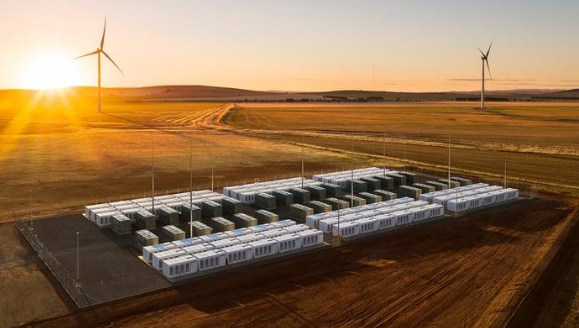
\includegraphics[width=6cm]{figures-Chp0/3-Reseau.png}
\end{minipage}\hfill   
\begin{minipage}[c]{0.35\textwidth}     
\captionof{figure}{Installation d'un centre de stockage d'énergie éolienne, par Tesla, en Australie exploité par le groupe français Neoen [tiré de la \href{https://www.maisondelenergie.fr/sites/maisondelenergie.fr/files/batteries_1.pdf}{maison de l'énergie, batteries}]}
\label{tab:battery_reseau}
\end{minipage}

\`{A} l'heure de la transition écologique, accompagnée du développement des énergies renouvelables, l'intégration des systèmes de stockage de masse au sein des réseaux électriques constitue un enjeu. En effet, les énergies renouvelables : photovoltaïque, éolien, nucléaire sont des sources d'énergies moins flexibles que le charbon ou le gaz. Les deux premières sont intermittentes (c.-à-d. dépendent des conditions environnementales) quand la dernière présente une production constante. Au sein du réseau électrique, l'intégration de batteries permet une meilleure maîtrise des pics ou des déficits de tension électrique.

\begin{comment}
\section{Objectifs du cours}

Il existe de multiples approches pour aborder les batteries, l'une des approches les plus communes est l'approche historique, consistant à décrire les avancées et les développements technologiques autour des batteries. Cette approche est celle utilisée par les chercheurs de renom du domaine comme J.M. Tarascon, professeur au collège de France, qui tient la chaire de Chimie du solide et énergie.

Cependant, cette approche nécessite souvent l'oeil aguéri d'un chimiste accompli dans la maîtrise des outils permettant d'aborder les batteries. Le domaine des matériaux pour l'énergie est un domaine transverse ! Toute la difficulté que vous allez rencontrer sera de faire appel à des notions de : chimie des solutions, de thermodynamique, de physique (électricité/électrostatique) à mettre en relation avec vos connaissances de chimie des matériaux. 

Dans ce cours, le choix a été fait de construire des chapitres/séances autour des "outils" permettant de comprendre cette branche des matériaux, sans aborder les développements technologiques actuels. Les outils développés en cours devront être réinvestis par vous lors des travaux dirigés qui présenteront des exercice de deux natures : 
\begin{enumerate}
\item des applications directes des outils du cours ; 
\item des problèmes plus complexes où vous serez emmené à aborder une technologie ancienne ou actuelle, à l'aide des outils développés en cours.
\end{enumerate}

Lors des séances de travaux pratiques, le choix a été fait de vous faire aborder les concepts élementaires autour des piles et batteries afin de vous familiariser avec les notions élémentaires de ces systèmes, puis de vous faire développer un système plus complexe : une batterie Li-ion, sous forme de "pile bouton".

\section{Organisation des séances}

\`{A} chaque séance, un outil sera abordé de manière théorique et formel. Un polycopié vous sera distribué, abordant le plus souvent le problème de manière conceptualisé et formalisé. Le cours, à l'oral, traitera le plus souvent un exemple type sur la base de laquelle l'outils sera développé et utilisé. Le polycopié et la séance orale sont donc complémentaires et ne peuvent être suivi l'un sans l'autre. Le polycopié est un bon moyen ensuite de revoir les notions abordées dans un cadre général.
\end{comment}